\section{Research Design}
\label{sec:research_design}

This research is inspired by the stated CB research approach and focuses on the development of 
the second CB element, an open simulation platform depicting the shared paradigm of LEM. 
The proposed design is presented in Figure \ref{figure:competitive_benchmarking}. 
In contrast to the initial CB research design, the third element CB Process differs. 
The platform enables research groups to design and test their artifacts in the field of the shared 
paradigm, using the developed platform. However, the designed artifacts in the form of autonomous 
software agents do not compete against each other in competitions. 
Rather, research groups can design and develop the behavior of all agents and the 
autonomous market mechanism. Hence, it is also possible to analyze and evaluate the designed 
artifacts and use them as a benchmark to compare different designs. 

\begin{figure}[htbp]
	\centering
	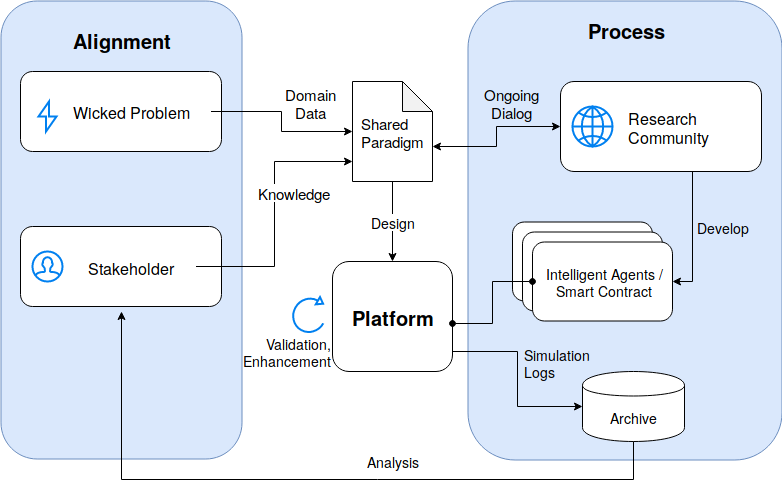
\includegraphics[width=1\linewidth]{./figures/competitive_benchmarking.png}
	\caption{Research Design following \protect\shortciteA{ketter2015competitive}}
	\label{figure:competitive_benchmarking}
\end{figure}

According to the IS Design Science principles introduced by \shortciteA{hevner2008design}, 
the presented research design produces a viable artifact in the form of an open simulation platform, which depicts a 
relevant real-world wicked problem. Due to the outcoming data produced by the simulation platform, 
it is possible to develop methods to evaluate the utility, quality, and efficacy of the artifact. 
Moreover, the research provides a verifiable contribution through the artifact, the open simulation platform, itself. 
The platform enables the investigation of possible solutions to unsolved problems and further, 
it removes the technical barriers for the use of the complex distributed ledger technology. 
Besides, the implementation of the platform is based on an appropriate selection of techniques. 
As stated in \ref{sec:Blockchain-based Energy Markets}, 
blockchains are a suitable technology to implement decentralized microgrid energy markets. 
In addition, the in \ref{sec:Distributed Resource Optimization} introduced BTM achieves evidentially system 
optimality under a dynamic market-trading algorithm. 
Therefore, this research relies upon the application of rigorous methods and comply with the requirement 
of the fifth guideline by \shortciteA{hevner2008design}. 
Besides, the platform enables the iterative search for an optimal design through the comparison 
of different produced solutions and is valuable to technology-oriented as well as management-oriented 
audiences. As a result, this research design also fulfills the seven research guidelines of 
the research framework introduced by \shortciteA{hevner2008design}. 
